\documentclass{article}

\usepackage[a4paper, total={6.5in, 11in}]{geometry}
\usepackage{graphicx}
\usepackage{subfig}
\usepackage{gensymb}
\usepackage{hyperref}
\graphicspath{{titech/CSC.T463.ComputerGraphics/h6/}}

\usepackage{latex/common}

\title{Computer Graphics 2021 - Assignment 6}
\author{Sixue Wang\\21M30927\\Tokyo Institute of Technology}

\begin{document}

\maketitle

\section{}

The vertices of an regular icosahedron centered at the origin with an edge length of 2 are
\begin{equation*}
  (0,\pm z,\pm x)
\end{equation*}
\begin{equation*}
  (\pm z,\pm x,0)
\end{equation*}
\begin{equation*}
  (\pm x,0,\pm z)
\end{equation*}
where $x = 1$, $z = \frac{1+\sqrt(5)}{2}$
For the icosahedron with edge length of 0.8, we can scale $x$ and $z$ by $0.4$.

The second step, translating and rotating, is similar with the previous assignment by modifing PMVMatrix.

\begin{figure}[h]
  \begin{tabular}{cc}
    \subfloat[]{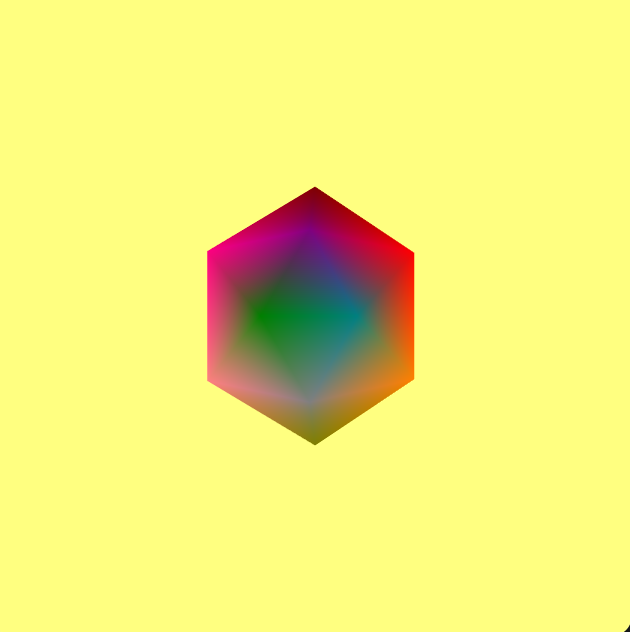
\includegraphics[width=0.3\textwidth]{h6_1.png}} &
    \subfloat[]{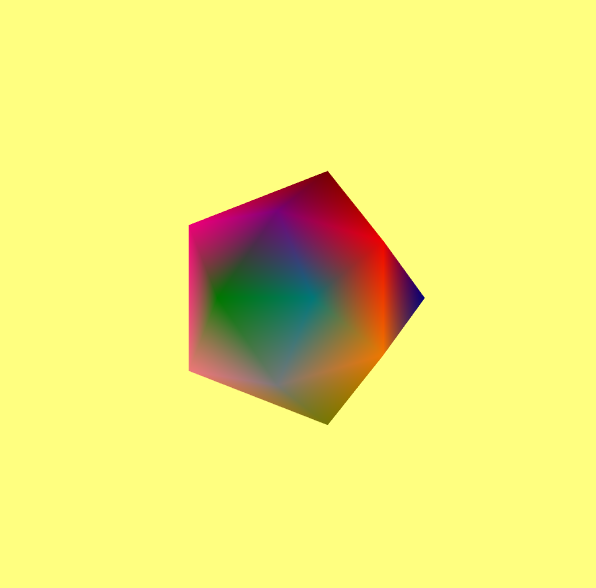
\includegraphics[width=0.3\textwidth]{h6_2.png}} \\
    \subfloat[]{
\includegraphics[width=0.3\textwidth]{h6_3.png}} &
    \subfloat[]{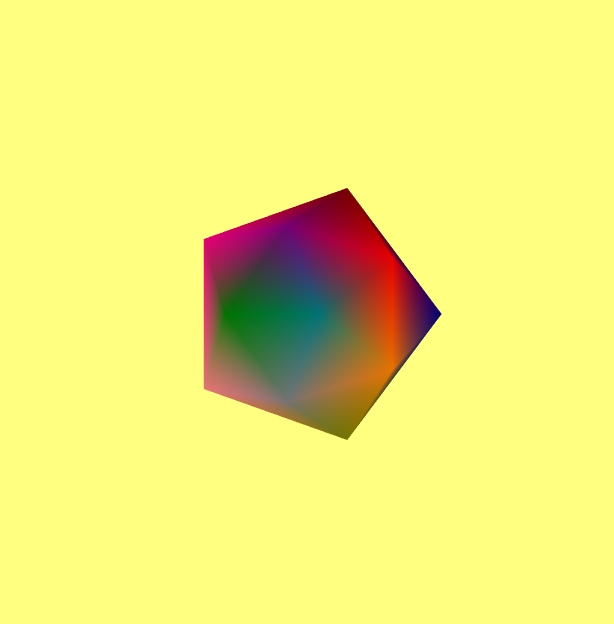
\includegraphics[width=0.3\textwidth]{h6_4.png}} \\
  \end{tabular}
\end{figure}

Another interesting thing is mapping texture to an icosahedron. In our case, we use the following equations:
\begin{equation*}
  u = \frac{atan(z, x)}{2PI}, v = \frac{asin(y)}{pi}+0.5
\end{equation*}

\section{}

To calculate normal directions of faces of icosahedron, we cannot directly use the normal attributes of vertices. We have to do it by:
\begin{center}
  normalize(inverse(transpose)(ModelView)) * normal
\end{center}
where the left term has been provided by the fourth matrix in PMVMatrix.

Then we place the light point at (0,0,10) and the camera at (2,5,-1) which used by specular reflection. According Phong reflection model, we combine ambient, diffuse, and specular reflection together(in spot.frag).

In our zip file, we also provided a screen record to show the result.

\section{Reference}
\begin{itemize}
  \item \href{https://en.wikipedia.org/wiki/Regular_icosahedron}{Regular icosahedron}: https://en.wikipedia.org/wiki/Regular\_icosahedronp
  \item \href{https://www.alexisgiard.com/icosahedron-sphere/}{Generating and UV mapping an icosahedron sphere}: https://www.alexisgiard.com/icosahedron-sphere/
  \item \href{https://www.youtube.com/watch?v=lH61rdpJ5v8}{OpenGL - lighting with the Phong reflection model (part 1 of 2)}: https://www.youtube.com/watch?v=lH61rdpJ5v8
  \item \href{https://www.youtube.com/watch?v=KdDdljGtfeg}{OpenGL - lighting with the Phong reflection model (part 2 of 2)}: https://www.youtube.com/watch?v=KdDdljGtfeg
\end{itemize}

\end{document}
